\documentclass{article}
\usepackage{amsfonts, amsthm, amsmath, amssymb, mathtools, ulem, mathrsfs, physics, esint, siunitx, tikz-cd}
\usepackage{pdfpages, fullpage, color, microtype, cancel, textcomp, markdown, hyperref, graphicx}
\usepackage{enumitem}
\usepackage{algorithm}
\usepackage{algpseudocode}
\graphicspath{{./images/}}
\usepackage[english]{babel}
\usepackage[autostyle, english=american]{csquotes}
\MakeOuterQuote{"}
\usepackage{xparse}
\usepackage{tikz}

\usepackage{calligra}
\DeclareMathAlphabet{\mathcalligra}{T1}{calligra}{m}{n}
\DeclareFontShape{T1}{calligra}{m}{n}{<->s*[2.2]callig15}{}
\newcommand{\script}[1]{\ensuremath{\mathcalligra{#1}}}
\newcommand{\scr}{\script r}

% fonts
\def\mbb#1{\mathbb{#1}}
\def\mfk#1{\mathfrak{#1}}
\def\mbf#1{\mathbf{#1}}
\def\tbf#1{\textbf{#1}}

% common bold letters
\def\bP{\mbb{P}}
\def\bC{\mbb{C}}
\def\bH{\mbb{H}}
\def\bI{\mbb{I}}
\def\bR{\mbb{R}}
\def\bQ{\mbb{Q}}
\def\bZ{\mbb{Z}}
\def\bN{\mbb{N}}

% brackets
\newcommand{\br}[1]{\left(#1\right)}
\newcommand{\sbr}[1]{\left[#1\right]}
\newcommand{\brc}[1]{\left\{#1\right\}}
\newcommand{\lbr}[1]{\left\langle#1\right\rangle}

% vectors
\renewcommand{\i}{\hat{\imath}}
\renewcommand{\j}{\hat{\jmath}}
\renewcommand{\k}{\hat{k}}
\newcommand{\proj}[2]{\text{proj}_{#2}\br{#1}}
\newcommand{\m}[2][b]{\begin{#1matrix}#2\end{#1matrix}}
\newcommand{\arr}[3][\sbr]{#1{\begin{array}{#2}#3\end{array}}}

% misc
\NewDocumentCommand{\seq}{O{n} O{1} O{\infty} m}{\br{#4}_{{#1}={#2}}^{#3}}
\NewDocumentCommand{\app}{O{x} O{\infty}}{\xrightarrow{#1\to#2}}
\newcommand{\sm}{\setminus}
\newcommand{\sse}{\subseteq}
\renewcommand{\ss}{\subset}
\newcommand{\vn}{\varnothing}
\newcommand{\lc}{\epsilon_{ijk}}
\newcommand{\ep}{\epsilon}
\newcommand{\vp}{\varphi}
\renewcommand{\th}{\theta}
\newcommand{\cjg}[1]{\overline{#1}}
\newcommand{\inv}{^{-1}}
\DeclareMathOperator{\im}{im}
\DeclareMathOperator{\id}{id}
\newcommand{\ans}{\tbf{Ans. }}
\newcommand{\pf}{\tbf{Pf. }}
\newcommand{\imp}{\implies}
\newcommand{\impleft}{\reflectbox{$\implies$}}
\newcommand{\ck}{\frac1{4\pi\ep_0}}
\newcommand{\ckb}{4\pi\ep_0}
\newcommand{\sto}{\longrightarrow}
\DeclareMathOperator{\cl}{cl}
\DeclareMathOperator{\intt}{int}
\DeclareMathOperator{\bd}{bd}
\DeclareMathOperator{\Span}{span}
\newcommand{\floor}[1]{\left\lfloor#1\right\rfloor}
\newcommand{\ceil}[1]{\left\lceil#1\right\rceil}
\newcommand{\fxn}[5]{#1:\begin{array}{rcl}#2&\longrightarrow & #3\\[-0.5mm]#4&\longmapsto &#5\end{array}}
\newcommand{\sep}[1][.5cm]{\vspace{#1}}
\DeclareMathOperator{\card}{card}
\renewcommand{\ip}[2]{\lbr{#1,#2}}
\renewcommand{\bar}{\overline}
\DeclareMathOperator{\cis}{cis}
\DeclareMathOperator{\Arg}{Arg}
\newcommand{\ptl}{\partial}

% title
\title{Scientific Computing HW 10}
\author{Ryan Chen}
%\date{\today}
\setlength{\parindent}{0pt}


\begin{document}
	
\maketitle



\tbf{Problem 1.}

\begin{enumerate}[label=(\alph*)]
	
\item Write $k_x=n\pi,~ky=m\pi$ where $1\le n,m\le J-1$, so that
$$v_{k_x,k_y}(x_r,y_s) = \sin n\pi x_r\sin m\pi y_s$$
Applying the discretized Laplace operator, we obtain
$$\frac{1}{h^2}\sbr{v|_{n+1,m}+v|_{n-1,m}+v|_{n,m+1}+v_{n,m-1}-4v|_{n,m}} \quad (1.1)$$
The bracked expression is
$$\sbr{\sin((n+1)\pi x_r)+\sin((n-1)\pi x_r)}\sin m\pi y_s + \sin n\pi x_r\sbr{\sin((m+1)\pi y_s)+\sin((m-1)\pi y_s)} - 4\sin n\pi x_r\sin m\pi y_s$$
Using the identity
$$\sin a + \sin b = 2\sin\frac{a+b}{2}\cos\frac{a-b}{2}$$
the bracked expression is
$$2\sin n\pi x_r\cos\pi x_r\si m\pi y_s + 2\sin m\pi y_s\cos\pi y_s\sin n\pi x_r - r\sin n\pi x_r\sin m\pi y_s$$
$$= \sin n\pi x_r\sin m\pi y_s\cdot 2\sbr{\cos\pi x_r+2\cos\pi y_s-2}$$
Hence the expression (1.1) equals
$$\sin n\pi x_r\sin m\pi y_s\cdot \frac{2}{h^2}\sbr{\cos\pi x_r+\cos\pi y_s-2}$$
We then see that the eigenvalues are
$$\lambda = \frac{2}{h^2}\sbr{\cos\pi x_r+\cos\pi y_s-2}$$


\item For stability, we demand that the eigenvalues of $\Delta tA$,
$$\lambda\Delta t = \frac{2\Delta t}{h^2}[\cos\pi x_r+\cos\pi y_s-2]$$
lie in the RAS of forward Euler, $[-2,0]$. Note that $-4\le\cos\pi x_r+\cos\pi y_s-2\le0$, hence
$$-2 \le \lambda\Delta t \le 0
\iff \frac{2\Delta t}{h^2} \le \frac12
\iff \Delta t \le \frac{h^2}{4}$$ 

\end{enumerate}
\pagebreak



\tbf{Problem 2.}

\begin{enumerate}[label=(\alph*)]
	
\item Fix a finite time $T$, integer $N$, and timestep $dt=\frac TN$. Using a scheme based on the trapezoidal rule,
$$u_{n+1} = u_n + \frac12dt(\Delta u_{n+1}+\Delta u_n) + dt
\imp u_{n+1} - \frac12dt\Delta u_{n+1} = dt + u_n + \frac12dt\Delta u_n$$
Fix a test function $v\in C^2(\Omega)$ with $v\eval_{\ptl\Omega}=0$. Multiply by $v$ and integrate over $\Omega$.
$$\int_\Omega u_{n+1}vdx - \frac12dt\int_\Omega v\Delta u_{n+1}dx = dt\int_\Omega vdx + \int_\Omega u_nvdx + \frac12dt\int_\Omega v\Delta u_ndx$$
Using Green's first identity and the fact $v|_{\ptl\Omega}=0$,
$$\int_\Omega v\Delta u_ndx = \int_{\ptl\Omega}v\pdv{u_n}{n}ds - \int_\Omega\grad v\cdot\grad u_ndx
= -\int_\Omega\grad v\cdot\grad u_ndx$$
and similarly for the term involving $\Delta u_{n+1}$. We obtain the weak solution to the IBVP.
$$\int_\Omega u_{n+1}vdx + \frac12dt\int_\Omega\grad v\cdot\grad u_{n+1}dx = dt\int_\Omega vdx + \int_\Omega u_nvdx + -\frac12dt\int_\Omega\grad v\cdot\grad u_ndx$$
From this we write the FEM solution. Given a triangulation $\tau$ of $\Omega$, let $\eta_i$ be the piecewise linear basis functions from prior FEM problems. Then for each timestep $n$, we solve 
$$\br{B+\frac12dtA}U_{n+1} = dtb + \br{B-\frac12dtA}U_n$$
where
$$A_{ij} = \int_\Omega\grad\eta_i\cdot\grad\eta_jdx,
\quad b_j = \int_\Omega\eta_jdx,
\quad B_{ij} = \int_\Omega\eta_i\eta_jdx$$


\item Code: \url{https://github.com/RokettoJanpu/Scientific-Computing-2/blob/main/hw10.ipynb}

We set a mesh for the annulus with center $(0,0)$, inner radius 1, and outer radius 2.

\begin{center}
	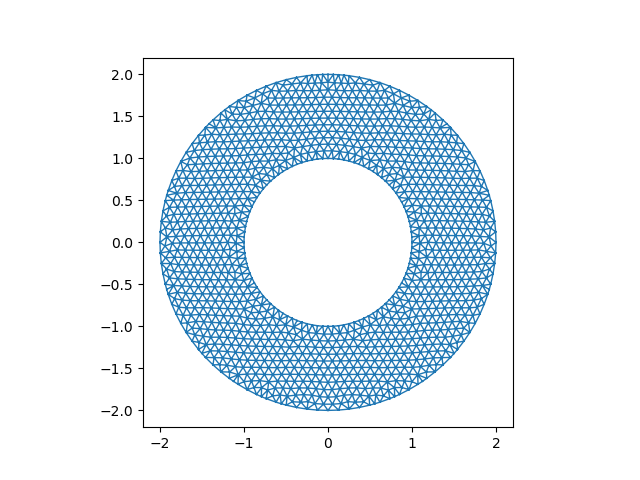
\includegraphics[scale=.6]{hw10 mesh}
\end{center}

Below is the numerical solution at $t=0.1$ and $t=1$.

\begin{center}
	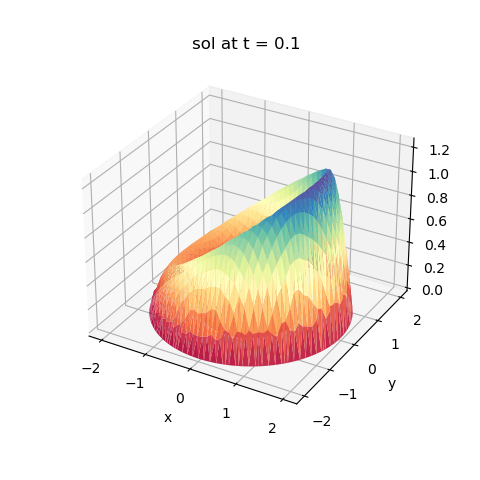
\includegraphics[scale=.6]{hw10 sol t=0.1}
	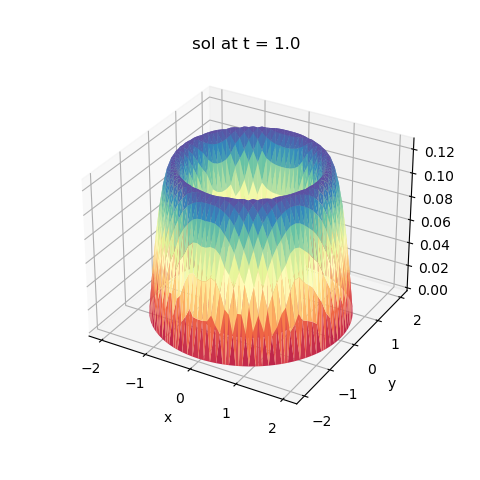
\includegraphics[scale=.6]{hw10 sol t=1.0}
\end{center}

Below are the steady state numerical and exact solutions plotted as functions of $r$. We see that the solutions essentially coincide.

\begin{center}
	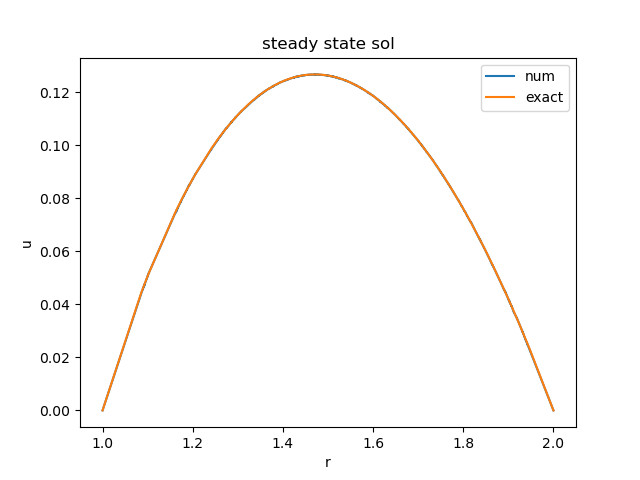
\includegraphics[scale=.6]{hw10 steady state sol}
\end{center}

\end{enumerate}


	
\end{document}